% Options for packages loaded elsewhere
\PassOptionsToPackage{unicode}{hyperref}
\PassOptionsToPackage{hyphens}{url}
\PassOptionsToPackage{dvipsnames,svgnames,x11names}{xcolor}
%
\documentclass[
  letterpaper,
  DIV=11,
  numbers=noendperiod]{scrartcl}

\usepackage{amsmath,amssymb}
\usepackage{iftex}
\ifPDFTeX
  \usepackage[T1]{fontenc}
  \usepackage[utf8]{inputenc}
  \usepackage{textcomp} % provide euro and other symbols
\else % if luatex or xetex
  \usepackage{unicode-math}
  \defaultfontfeatures{Scale=MatchLowercase}
  \defaultfontfeatures[\rmfamily]{Ligatures=TeX,Scale=1}
\fi
\usepackage{lmodern}
\ifPDFTeX\else  
    % xetex/luatex font selection
\fi
% Use upquote if available, for straight quotes in verbatim environments
\IfFileExists{upquote.sty}{\usepackage{upquote}}{}
\IfFileExists{microtype.sty}{% use microtype if available
  \usepackage[]{microtype}
  \UseMicrotypeSet[protrusion]{basicmath} % disable protrusion for tt fonts
}{}
\makeatletter
\@ifundefined{KOMAClassName}{% if non-KOMA class
  \IfFileExists{parskip.sty}{%
    \usepackage{parskip}
  }{% else
    \setlength{\parindent}{0pt}
    \setlength{\parskip}{6pt plus 2pt minus 1pt}}
}{% if KOMA class
  \KOMAoptions{parskip=half}}
\makeatother
\usepackage{xcolor}
\setlength{\emergencystretch}{3em} % prevent overfull lines
\setcounter{secnumdepth}{-\maxdimen} % remove section numbering
% Make \paragraph and \subparagraph free-standing
\ifx\paragraph\undefined\else
  \let\oldparagraph\paragraph
  \renewcommand{\paragraph}[1]{\oldparagraph{#1}\mbox{}}
\fi
\ifx\subparagraph\undefined\else
  \let\oldsubparagraph\subparagraph
  \renewcommand{\subparagraph}[1]{\oldsubparagraph{#1}\mbox{}}
\fi

\usepackage{color}
\usepackage{fancyvrb}
\newcommand{\VerbBar}{|}
\newcommand{\VERB}{\Verb[commandchars=\\\{\}]}
\DefineVerbatimEnvironment{Highlighting}{Verbatim}{commandchars=\\\{\}}
% Add ',fontsize=\small' for more characters per line
\usepackage{framed}
\definecolor{shadecolor}{RGB}{241,243,245}
\newenvironment{Shaded}{\begin{snugshade}}{\end{snugshade}}
\newcommand{\AlertTok}[1]{\textcolor[rgb]{0.68,0.00,0.00}{#1}}
\newcommand{\AnnotationTok}[1]{\textcolor[rgb]{0.37,0.37,0.37}{#1}}
\newcommand{\AttributeTok}[1]{\textcolor[rgb]{0.40,0.45,0.13}{#1}}
\newcommand{\BaseNTok}[1]{\textcolor[rgb]{0.68,0.00,0.00}{#1}}
\newcommand{\BuiltInTok}[1]{\textcolor[rgb]{0.00,0.23,0.31}{#1}}
\newcommand{\CharTok}[1]{\textcolor[rgb]{0.13,0.47,0.30}{#1}}
\newcommand{\CommentTok}[1]{\textcolor[rgb]{0.37,0.37,0.37}{#1}}
\newcommand{\CommentVarTok}[1]{\textcolor[rgb]{0.37,0.37,0.37}{\textit{#1}}}
\newcommand{\ConstantTok}[1]{\textcolor[rgb]{0.56,0.35,0.01}{#1}}
\newcommand{\ControlFlowTok}[1]{\textcolor[rgb]{0.00,0.23,0.31}{#1}}
\newcommand{\DataTypeTok}[1]{\textcolor[rgb]{0.68,0.00,0.00}{#1}}
\newcommand{\DecValTok}[1]{\textcolor[rgb]{0.68,0.00,0.00}{#1}}
\newcommand{\DocumentationTok}[1]{\textcolor[rgb]{0.37,0.37,0.37}{\textit{#1}}}
\newcommand{\ErrorTok}[1]{\textcolor[rgb]{0.68,0.00,0.00}{#1}}
\newcommand{\ExtensionTok}[1]{\textcolor[rgb]{0.00,0.23,0.31}{#1}}
\newcommand{\FloatTok}[1]{\textcolor[rgb]{0.68,0.00,0.00}{#1}}
\newcommand{\FunctionTok}[1]{\textcolor[rgb]{0.28,0.35,0.67}{#1}}
\newcommand{\ImportTok}[1]{\textcolor[rgb]{0.00,0.46,0.62}{#1}}
\newcommand{\InformationTok}[1]{\textcolor[rgb]{0.37,0.37,0.37}{#1}}
\newcommand{\KeywordTok}[1]{\textcolor[rgb]{0.00,0.23,0.31}{#1}}
\newcommand{\NormalTok}[1]{\textcolor[rgb]{0.00,0.23,0.31}{#1}}
\newcommand{\OperatorTok}[1]{\textcolor[rgb]{0.37,0.37,0.37}{#1}}
\newcommand{\OtherTok}[1]{\textcolor[rgb]{0.00,0.23,0.31}{#1}}
\newcommand{\PreprocessorTok}[1]{\textcolor[rgb]{0.68,0.00,0.00}{#1}}
\newcommand{\RegionMarkerTok}[1]{\textcolor[rgb]{0.00,0.23,0.31}{#1}}
\newcommand{\SpecialCharTok}[1]{\textcolor[rgb]{0.37,0.37,0.37}{#1}}
\newcommand{\SpecialStringTok}[1]{\textcolor[rgb]{0.13,0.47,0.30}{#1}}
\newcommand{\StringTok}[1]{\textcolor[rgb]{0.13,0.47,0.30}{#1}}
\newcommand{\VariableTok}[1]{\textcolor[rgb]{0.07,0.07,0.07}{#1}}
\newcommand{\VerbatimStringTok}[1]{\textcolor[rgb]{0.13,0.47,0.30}{#1}}
\newcommand{\WarningTok}[1]{\textcolor[rgb]{0.37,0.37,0.37}{\textit{#1}}}

\providecommand{\tightlist}{%
  \setlength{\itemsep}{0pt}\setlength{\parskip}{0pt}}\usepackage{longtable,booktabs,array}
\usepackage{calc} % for calculating minipage widths
% Correct order of tables after \paragraph or \subparagraph
\usepackage{etoolbox}
\makeatletter
\patchcmd\longtable{\par}{\if@noskipsec\mbox{}\fi\par}{}{}
\makeatother
% Allow footnotes in longtable head/foot
\IfFileExists{footnotehyper.sty}{\usepackage{footnotehyper}}{\usepackage{footnote}}
\makesavenoteenv{longtable}
\usepackage{graphicx}
\makeatletter
\def\maxwidth{\ifdim\Gin@nat@width>\linewidth\linewidth\else\Gin@nat@width\fi}
\def\maxheight{\ifdim\Gin@nat@height>\textheight\textheight\else\Gin@nat@height\fi}
\makeatother
% Scale images if necessary, so that they will not overflow the page
% margins by default, and it is still possible to overwrite the defaults
% using explicit options in \includegraphics[width, height, ...]{}
\setkeys{Gin}{width=\maxwidth,height=\maxheight,keepaspectratio}
% Set default figure placement to htbp
\makeatletter
\def\fps@figure{htbp}
\makeatother

\KOMAoption{captions}{tableheading}
\makeatletter
\@ifpackageloaded{caption}{}{\usepackage{caption}}
\AtBeginDocument{%
\ifdefined\contentsname
  \renewcommand*\contentsname{Table of contents}
\else
  \newcommand\contentsname{Table of contents}
\fi
\ifdefined\listfigurename
  \renewcommand*\listfigurename{List of Figures}
\else
  \newcommand\listfigurename{List of Figures}
\fi
\ifdefined\listtablename
  \renewcommand*\listtablename{List of Tables}
\else
  \newcommand\listtablename{List of Tables}
\fi
\ifdefined\figurename
  \renewcommand*\figurename{Figure}
\else
  \newcommand\figurename{Figure}
\fi
\ifdefined\tablename
  \renewcommand*\tablename{Table}
\else
  \newcommand\tablename{Table}
\fi
}
\@ifpackageloaded{float}{}{\usepackage{float}}
\floatstyle{ruled}
\@ifundefined{c@chapter}{\newfloat{codelisting}{h}{lop}}{\newfloat{codelisting}{h}{lop}[chapter]}
\floatname{codelisting}{Listing}
\newcommand*\listoflistings{\listof{codelisting}{List of Listings}}
\makeatother
\makeatletter
\makeatother
\makeatletter
\@ifpackageloaded{caption}{}{\usepackage{caption}}
\@ifpackageloaded{subcaption}{}{\usepackage{subcaption}}
\makeatother
\ifLuaTeX
  \usepackage{selnolig}  % disable illegal ligatures
\fi
\usepackage{bookmark}

\IfFileExists{xurl.sty}{\usepackage{xurl}}{} % add URL line breaks if available
\urlstyle{same} % disable monospaced font for URLs
\hypersetup{
  pdftitle={Exploratory Data Analysis},
  pdfauthor={Saniya Bekova},
  colorlinks=true,
  linkcolor={blue},
  filecolor={Maroon},
  citecolor={Blue},
  urlcolor={Blue},
  pdfcreator={LaTeX via pandoc}}

\title{Exploratory Data Analysis}
\author{Saniya Bekova}
\date{2024-10-14}

\begin{document}
\maketitle

\begin{Shaded}
\begin{Highlighting}[]
\CommentTok{\#load necessary libraries}
\FunctionTok{library}\NormalTok{(tidyverse)}
\FunctionTok{library}\NormalTok{(readxl)}
\FunctionTok{library}\NormalTok{(haven) }\CommentTok{\#for loading other datafiles (SAS, STATA, SPSS, etc.)}
\FunctionTok{library}\NormalTok{(stringr)}
\FunctionTok{library}\NormalTok{(lubridate)}
\FunctionTok{library}\NormalTok{(ggplot2)}
\FunctionTok{library}\NormalTok{(dplyr)}
\FunctionTok{library}\NormalTok{(ggrepel)}
\FunctionTok{library}\NormalTok{(scales)}
\FunctionTok{library}\NormalTok{(tidymodels)}
\end{Highlighting}
\end{Shaded}

\begin{Shaded}
\begin{Highlighting}[]
\CommentTok{\#load data}
\NormalTok{education\_data }\OtherTok{\textless{}{-}} \FunctionTok{read\_csv}\NormalTok{(}\StringTok{\textquotesingle{}data/education\_data.csv\textquotesingle{}}\NormalTok{)  }\CommentTok{\# Dataset 1: Educational indicators}
\NormalTok{imo\_data }\OtherTok{\textless{}{-}} \FunctionTok{read\_csv}\NormalTok{(}\StringTok{\textquotesingle{}data/imo\_data.csv\textquotesingle{}}\NormalTok{)  }\CommentTok{\# Dataset 2: IMO competition results}
\end{Highlighting}
\end{Shaded}

\subsection{Main Outcome/Target (Y
Variable):}\label{main-outcometarget-y-variable}

The main outcome or target variable in this analysis is the
\textbf{average score per contestant for each country in a given year}.
This is calculated by summing the scores from problems 1 to 7 for each
country's team and dividing the total by the number of participants
(team\_size\_all). This variable represents how well the entire team
from each country performed in the International Mathematical Olympiad
(IMO).

This outcome is a good fit for the study because it provides a clear
measure of how well a country's education system prepares students for
international competitions. By using the average score, the analysis
captures the performance of the whole team, not just the top individual
performers. This is important for understanding the impact of
educational investments, such as government spending on education,
literacy rates, and school completion rates, on a country's success in
the IMO.

The average score per contestant gives a more detailed and fair
comparison between countries. It helps to evaluate the overall strength
of the team, making it a useful measure for examining how education
systems contribute to performance in international competitions.

By focusing on the average score, this analysis can effectively explore
the connection between educational investments and a country's overall
performance in the IMO, making it a suitable target for this project.

\subsection{Data Cleaning}\label{data-cleaning}

\begin{Shaded}
\begin{Highlighting}[]
\NormalTok{literacy\_rate\_by\_country\_and\_region }\OtherTok{\textless{}{-}} \FunctionTok{read\_csv}\NormalTok{(}\StringTok{"data/literacy\_data.csv"}\NormalTok{)}

\NormalTok{country\_and\_region\_data }\OtherTok{\textless{}{-}} \FunctionTok{read\_xlsx}\NormalTok{(}\StringTok{"data/P\_Data\_Extract\_From\_Education\_Statistics\_{-}\_All\_Indicators\_Metadata.xlsx"}\NormalTok{, }\AttributeTok{sheet =} \StringTok{"Country {-} Metadata"}\NormalTok{)}

\NormalTok{youth\_literacy\_rate }\OtherTok{\textless{}{-}}\NormalTok{ literacy\_rate\_by\_country\_and\_region }\SpecialCharTok{|\textgreater{}}
  \FunctionTok{filter}\NormalTok{(Series }\SpecialCharTok{==} \StringTok{"Youth literacy rate, population 15{-}24 years, both sexes (\%)"}\NormalTok{)}

\NormalTok{youth\_literacy\_rate }\OtherTok{\textless{}{-}} \FunctionTok{pivot\_longer}\NormalTok{(youth\_literacy\_rate, }
                                   \AttributeTok{cols =} \FunctionTok{c}\NormalTok{(}\StringTok{\textquotesingle{}2009 [YR2009]\textquotesingle{}}\NormalTok{, }\StringTok{\textquotesingle{}2010 [YR2010]\textquotesingle{}}\NormalTok{, }\StringTok{\textquotesingle{}2011 [YR2011]\textquotesingle{}}\NormalTok{, }\StringTok{\textquotesingle{}2012 [YR2012]\textquotesingle{}}\NormalTok{, }\StringTok{\textquotesingle{}2013 [YR2013]\textquotesingle{}}\NormalTok{, }\StringTok{\textquotesingle{}2014 [YR2014]\textquotesingle{}}\NormalTok{, }\StringTok{\textquotesingle{}2015 [YR2015]\textquotesingle{}}\NormalTok{, }\StringTok{\textquotesingle{}2016 [YR2016]\textquotesingle{}}\NormalTok{, }\StringTok{\textquotesingle{}2017 [YR2017]\textquotesingle{}}\NormalTok{, }\StringTok{\textquotesingle{}2018 [YR2018]\textquotesingle{}}\NormalTok{, }\StringTok{\textquotesingle{}2019 [YR2019]\textquotesingle{}}\NormalTok{), }
                                   \AttributeTok{names\_to =} \StringTok{"Year"}\NormalTok{,                  }
                                   \AttributeTok{values\_to =} \StringTok{"Literacy\_Rate"}\NormalTok{) }\SpecialCharTok{|\textgreater{}}
  \FunctionTok{mutate}\NormalTok{(}\AttributeTok{Year =} \FunctionTok{str\_replace}\NormalTok{(Year, }\StringTok{" }\SpecialCharTok{\textbackslash{}\textbackslash{}}\StringTok{[YR[0{-}9]+}\SpecialCharTok{\textbackslash{}\textbackslash{}}\StringTok{]"}\NormalTok{, }\StringTok{""}\NormalTok{)) }\SpecialCharTok{|\textgreater{}}
  \FunctionTok{select}\NormalTok{(}\StringTok{"Country Code"}\NormalTok{, }\StringTok{"Country Name"}\NormalTok{, Year, Literacy\_Rate)}

\NormalTok{youth\_literacy\_rate }\OtherTok{\textless{}{-}}\NormalTok{ youth\_literacy\_rate }\SpecialCharTok{|\textgreater{}}
  \FunctionTok{mutate}\NormalTok{(}\AttributeTok{Year =} \FunctionTok{as.double}\NormalTok{(Year),}
         \AttributeTok{Literacy\_Rate =} \FunctionTok{as.double}\NormalTok{(Literacy\_Rate))}


\NormalTok{education\_data\_joined }\OtherTok{\textless{}{-}}\NormalTok{ education\_data }\SpecialCharTok{|\textgreater{}}
  \FunctionTok{left\_join}\NormalTok{(youth\_literacy\_rate, }
            \AttributeTok{by =} \FunctionTok{c}\NormalTok{(}\StringTok{"Country"} \OtherTok{=} \StringTok{"Country Name"}\NormalTok{, }\StringTok{"Year"} \OtherTok{=} \StringTok{"Year"}\NormalTok{), }
            \AttributeTok{suffix =} \FunctionTok{c}\NormalTok{(}\StringTok{""}\NormalTok{, }\StringTok{"\_new"}\NormalTok{))}

\NormalTok{education\_data\_updated }\OtherTok{\textless{}{-}}\NormalTok{ education\_data\_joined }\SpecialCharTok{|\textgreater{}}
  \FunctionTok{mutate}\NormalTok{(}\AttributeTok{Value\_literacy\_rate =} \FunctionTok{coalesce}\NormalTok{(Value\_literacy\_rate, }
\NormalTok{                                        Literacy\_Rate)) }\SpecialCharTok{|\textgreater{}}
  \FunctionTok{select}\NormalTok{(}\SpecialCharTok{{-}}\NormalTok{Literacy\_Rate)}
\end{Highlighting}
\end{Shaded}

\begin{Shaded}
\begin{Highlighting}[]
\NormalTok{education\_with\_region }\OtherTok{\textless{}{-}}\NormalTok{ education\_data\_updated }\SpecialCharTok{|\textgreater{}}
  \FunctionTok{left\_join}\NormalTok{(country\_and\_region\_data, }\AttributeTok{by =} \FunctionTok{c}\NormalTok{(}\StringTok{"Country"} \OtherTok{=} \StringTok{"Long Name"}\NormalTok{))}

\NormalTok{education\_full }\OtherTok{\textless{}{-}}\NormalTok{ education\_with\_region }\SpecialCharTok{|\textgreater{}}
  \FunctionTok{left\_join}\NormalTok{(youth\_literacy\_rate, }
            \AttributeTok{by =} \FunctionTok{c}\NormalTok{(}\StringTok{"Region"} \OtherTok{=} \StringTok{"Country Name"}\NormalTok{, }\StringTok{"Year"} \OtherTok{=} \StringTok{"Year"}\NormalTok{),  }
            \AttributeTok{suffix =} \FunctionTok{c}\NormalTok{(}\StringTok{""}\NormalTok{, }\StringTok{"\_region"}\NormalTok{)) }\SpecialCharTok{|\textgreater{}}
  \FunctionTok{left\_join}\NormalTok{(youth\_literacy\_rate, }
            \AttributeTok{by =} \FunctionTok{c}\NormalTok{(}\StringTok{"Country"} \OtherTok{=} \StringTok{"Country Name"}\NormalTok{, }\StringTok{"Year"} \OtherTok{=} \StringTok{"Year"}\NormalTok{), }
            \AttributeTok{suffix =} \FunctionTok{c}\NormalTok{(}\StringTok{""}\NormalTok{, }\StringTok{"\_country"}\NormalTok{)) }\SpecialCharTok{|\textgreater{}}
  \FunctionTok{left\_join}\NormalTok{(youth\_literacy\_rate,}
            \AttributeTok{by =} \FunctionTok{c}\NormalTok{(}\StringTok{"Income Group"} \OtherTok{=} \StringTok{"Country Name"}\NormalTok{, }\StringTok{"Year"} \OtherTok{=} \StringTok{"Year"}\NormalTok{), }
            \AttributeTok{suffix =} \FunctionTok{c}\NormalTok{(}\StringTok{""}\NormalTok{, }\StringTok{"\_income"}\NormalTok{))}

\NormalTok{education\_data\_updated }\OtherTok{\textless{}{-}}\NormalTok{ education\_full }\SpecialCharTok{|\textgreater{}}
  \FunctionTok{mutate}\NormalTok{(}\AttributeTok{Value\_literacy\_rate =} \FunctionTok{coalesce}\NormalTok{(Value\_literacy\_rate, }
\NormalTok{                                        Literacy\_Rate\_country, }
\NormalTok{                                        Literacy\_Rate)) }\SpecialCharTok{|\textgreater{}}
  \FunctionTok{select}\NormalTok{(}\SpecialCharTok{{-}}\NormalTok{Literacy\_Rate\_country, }\SpecialCharTok{{-}}\NormalTok{Literacy\_Rate)  }

\NormalTok{education\_data\_updated }\OtherTok{\textless{}{-}}\NormalTok{ education\_data\_updated }\SpecialCharTok{|\textgreater{}}
  \FunctionTok{mutate}\NormalTok{(}\AttributeTok{Value\_literacy\_rate =} \FunctionTok{coalesce}\NormalTok{(Value\_literacy\_rate, }
\NormalTok{                                        Literacy\_Rate\_income)) }\SpecialCharTok{|\textgreater{}}
  \FunctionTok{select}\NormalTok{(Country, }
\NormalTok{         Year, }
         \StringTok{\textasciigrave{}}\AttributeTok{Country Code}\StringTok{\textasciigrave{}}\NormalTok{, }
\NormalTok{         Value\_gross\_enr\_ratio\_for\_tertirary\_edu,}
\NormalTok{         Value\_gov\_expen\_as\_perc\_of\_GPP, }
\NormalTok{         Value\_literacy\_rate, }
\NormalTok{         Region, }
         \StringTok{\textasciigrave{}}\AttributeTok{Income Group}\StringTok{\textasciigrave{}}\NormalTok{)}
\end{Highlighting}
\end{Shaded}

Merging Educational Data:

The educational indicators from the UNESCO Institute for Statistics were
split across multiple variables (e.g., primary and secondary education
completion rates, government expenditure on education). These were
merged into a single dataset, ensuring all relevant indicators were
available for each country and year. The merging process involved
handling mismatched country names between the datasets. For example,
differences such as ``Kyrgyz Republic'' vs.~``Kyrgyzstan'' were
corrected manually to ensure proper alignment of the data.

Combining IMO Data with Educational Data:

The educational data (which now included literacy rates, completion
rates, and government expenditure) was merged with the IMO performance
data (e.g., team scores, medals won) to create a comprehensive dataset.
This allowed for the analysis of the relationship between a country's
educational indicators and its performance in the IMO.

\subsection{Creating New Variables :}\label{creating-new-variables}

\texttt{Medal\_Efficiency} This variable was created by dividing the
total number of medals (gold, silver, and bronze) won by a country by
its team size (team\_size\_all). It measures how efficiently a country
converts its team into medals, providing insights into performance
relative to team size.

\texttt{Gov\_Investment\_Per\_Medal} This variable measures the amount
of government expenditure on education required to produce one IMO
medal. It was created by dividing the government expenditure as a
percentage of GDP by the total number of medals won.

\texttt{Lit\_Performance\_Ratio} This variable measures the ratio
between a country's youth literacy rate and its average IMO score or
total number of medals won, helping to explore the link between literacy
and performance.

These variables were created before the training-test split to avoid any
issues related to leakage between the datasets.

\begin{Shaded}
\begin{Highlighting}[]
\CommentTok{\# Calculate total score by summing problem scores p1 to p7}
\NormalTok{imo\_data }\OtherTok{\textless{}{-}}\NormalTok{ imo\_data }\SpecialCharTok{|\textgreater{}}
  \FunctionTok{rowwise}\NormalTok{() }\SpecialCharTok{|\textgreater{}}
  \FunctionTok{mutate}\NormalTok{(}\AttributeTok{total\_score =} \FunctionTok{sum}\NormalTok{(}\FunctionTok{c\_across}\NormalTok{(p1}\SpecialCharTok{:}\NormalTok{p7), }\AttributeTok{na.rm =} \ConstantTok{TRUE}\NormalTok{)) }\SpecialCharTok{|\textgreater{}}
  \FunctionTok{ungroup}\NormalTok{()  }

\CommentTok{\# Calculate average score per contestant by dividing total score by team size}
\NormalTok{imo\_data }\OtherTok{\textless{}{-}}\NormalTok{ imo\_data }\SpecialCharTok{|\textgreater{}}
  \FunctionTok{mutate}\NormalTok{(}\AttributeTok{average\_score\_per\_contestant =}\NormalTok{ total\_score }\SpecialCharTok{/}\NormalTok{ team\_size\_all)}

\NormalTok{imo\_data }\OtherTok{\textless{}{-}}\NormalTok{ imo\_data }\SpecialCharTok{|\textgreater{}}
  \FunctionTok{mutate}\NormalTok{(}\AttributeTok{medal\_Efficiency =} \FunctionTok{ifelse}\NormalTok{(team\_size\_all }\SpecialCharTok{\textgreater{}} \DecValTok{0}\NormalTok{, }
\NormalTok{                                   (awards\_gold }\SpecialCharTok{+}\NormalTok{ awards\_silver }\SpecialCharTok{+}\NormalTok{ awards\_bronze) }\SpecialCharTok{/}\NormalTok{ team\_size\_all, }
                                   \ConstantTok{NA}\NormalTok{))}

\CommentTok{\# Merging \textquotesingle{}imo\_data\textquotesingle{} with \textquotesingle{}education\_data\_updated\textquotesingle{}}
\NormalTok{combined\_data }\OtherTok{\textless{}{-}}\NormalTok{ imo\_data }\SpecialCharTok{|\textgreater{}}
  \FunctionTok{left\_join}\NormalTok{(education\_data\_updated, }\AttributeTok{by =} \FunctionTok{c}\NormalTok{(}\StringTok{"country"} \OtherTok{=} \StringTok{"Country"}\NormalTok{, }\StringTok{"year"} \OtherTok{=} \StringTok{"Year"}\NormalTok{))}

\NormalTok{combined\_data }\OtherTok{\textless{}{-}}\NormalTok{ combined\_data }\SpecialCharTok{|\textgreater{}}
  \FunctionTok{mutate}\NormalTok{(}\AttributeTok{Gov\_Investment\_Per\_Medal =} \FunctionTok{ifelse}\NormalTok{((awards\_gold }\SpecialCharTok{+}\NormalTok{ awards\_silver }\SpecialCharTok{+}\NormalTok{ awards\_bronze) }\SpecialCharTok{\textgreater{}} \DecValTok{0}\NormalTok{, }
\NormalTok{                                           Value\_gov\_expen\_as\_perc\_of\_GPP }\SpecialCharTok{/}\NormalTok{ (awards\_gold }\SpecialCharTok{+}\NormalTok{ awards\_silver }\SpecialCharTok{+}\NormalTok{ awards\_bronze), }
                                           \ConstantTok{NA}\NormalTok{),}
         \AttributeTok{Lit\_Performance\_Ratio =} \FunctionTok{ifelse}\NormalTok{(average\_score\_per\_contestant }\SpecialCharTok{\textgreater{}} \DecValTok{0}\NormalTok{, }
\NormalTok{                                        Value\_literacy\_rate }\SpecialCharTok{/}\NormalTok{ average\_score\_per\_contestant, }
                                        \ConstantTok{NA}\NormalTok{))}

\NormalTok{combined\_data }\OtherTok{\textless{}{-}}\NormalTok{ combined\_data }\SpecialCharTok{|\textgreater{}}
  \FunctionTok{filter}\NormalTok{(year }\SpecialCharTok{\textgreater{}} \DecValTok{2008} \SpecialCharTok{\&}\NormalTok{ year }\SpecialCharTok{\textless{}} \DecValTok{2020}\NormalTok{)}


\FunctionTok{summary}\NormalTok{(combined\_data)}
\end{Highlighting}
\end{Shaded}

\begin{verbatim}
      year        country          team_size_all   team_size_male 
 Min.   :2009   Length:1142        Min.   :1.000   Min.   :1.000  
 1st Qu.:2011   Class :character   1st Qu.:6.000   1st Qu.:5.000  
 Median :2014   Mode  :character   Median :6.000   Median :5.000  
 Mean   :2014                      Mean   :5.511   Mean   :5.001  
 3rd Qu.:2017                      3rd Qu.:6.000   3rd Qu.:6.000  
 Max.   :2019                      Max.   :6.000   Max.   :6.000  
                                                   NA's   :11     
 team_size_female       p1              p2              p3        
 Min.   :1.000    Min.   : 0.00   Min.   : 0.00   Min.   : 0.000  
 1st Qu.:1.000    1st Qu.:17.00   1st Qu.: 2.00   1st Qu.: 0.000  
 Median :1.000    Median :34.00   Median : 9.00   Median : 0.000  
 Mean   :1.331    Mean   :28.25   Mean   :13.01   Mean   : 2.986  
 3rd Qu.:2.000    3rd Qu.:41.00   3rd Qu.:22.00   3rd Qu.: 3.000  
 Max.   :6.000    Max.   :42.00   Max.   :42.00   Max.   :42.000  
 NA's   :668      NA's   :1       NA's   :1       NA's   :1       
       p4              p5              p6            p7         
 Min.   : 0.00   Min.   : 0.00   Min.   : 0.000   Mode:logical  
 1st Qu.:11.00   1st Qu.: 2.00   1st Qu.: 0.000   NA's:1142     
 Median :26.00   Median : 7.00   Median : 0.000                 
 Mean   :24.47   Mean   :11.54   Mean   : 2.186                 
 3rd Qu.:39.00   3rd Qu.:18.00   3rd Qu.: 2.000                 
 Max.   :42.00   Max.   :42.00   Max.   :36.000                 
 NA's   :1       NA's   :1       NA's   :1                      
  awards_gold    awards_silver    awards_bronze   awards_honorable_mentions
 Min.   :0.000   Min.   :0.0000   Min.   :0.000   Min.   :0.000            
 1st Qu.:0.000   1st Qu.:0.0000   1st Qu.:0.000   1st Qu.:0.000            
 Median :0.000   Median :0.0000   Median :1.000   Median :1.000            
 Mean   :0.461   Mean   :0.9351   Mean   :1.339   Mean   :1.409            
 3rd Qu.:0.000   3rd Qu.:2.0000   3rd Qu.:2.000   3rd Qu.:2.000            
 Max.   :6.000   Max.   :6.0000   Max.   :6.000   Max.   :6.000            
 NA's   :1       NA's   :1        NA's   :1       NA's   :1                
    leader          deputy_leader       total_score    
 Length:1142        Length:1142        Min.   :  0.00  
 Class :character   Class :character   1st Qu.: 39.25  
 Mode  :character   Mode  :character   Median : 79.00  
                                       Mean   : 82.37  
                                       3rd Qu.:119.75  
                                       Max.   :227.00  
                                                       
 average_score_per_contestant medal_Efficiency Country Code      
 Min.   : 0.000               Min.   :0.0000   Length:1142       
 1st Qu.: 8.167               1st Qu.:0.0000   Class :character  
 Median :13.667               Median :0.4000   Mode  :character  
 Mean   :14.350               Mean   :0.4689                     
 3rd Qu.:20.000               3rd Qu.:0.8333                     
 Max.   :37.833               Max.   :1.0000                     
                              NA's   :1                          
 Value_gross_enr_ratio_for_tertirary_edu Value_gov_expen_as_perc_of_GPP
 Min.   :  4.02                          Min.   : 0.390                
 1st Qu.: 37.49                          1st Qu.: 3.540                
 Median : 59.18                          Median : 4.520                
 Mean   : 56.98                          Mean   : 4.564                
 3rd Qu.: 77.23                          3rd Qu.: 5.450                
 Max.   :143.96                          Max.   :10.670                
 NA's   :573                             NA's   :573                   
 Value_literacy_rate    Region          Income Group      
 Min.   : 50.00      Length:1142        Length:1142       
 1st Qu.: 98.25      Class :character   Class :character  
 Median : 99.57      Mode  :character   Mode  :character  
 Mean   : 96.77                                           
 3rd Qu.: 99.66                                           
 Max.   :100.00                                           
 NA's   :571                                              
 Gov_Investment_Per_Medal Lit_Performance_Ratio
 Min.   :0.160            Min.   :  2.620      
 1st Qu.:0.780            1st Qu.:  5.054      
 Median :1.126            Median :  7.470      
 Mean   :1.969            Mean   : 15.681      
 3rd Qu.:2.632            3rd Qu.: 12.208      
 Max.   :8.960            Max.   :446.425      
 NA's   :718              NA's   :575          
\end{verbatim}

\begin{Shaded}
\begin{Highlighting}[]
\FunctionTok{write\_csv}\NormalTok{(combined\_data, }\StringTok{"data/combined\_data.csv"}\NormalTok{)}
\end{Highlighting}
\end{Shaded}

\subsection{Split data}\label{split-data}

\begin{Shaded}
\begin{Highlighting}[]
\FunctionTok{set.seed}\NormalTok{(}\DecValTok{1234}\NormalTok{)}
\NormalTok{combined\_data\_split }\OtherTok{\textless{}{-}} \FunctionTok{initial\_split}\NormalTok{(combined\_data, }\AttributeTok{prop =} \DecValTok{3}\SpecialCharTok{/}\DecValTok{4}\NormalTok{, }\AttributeTok{strata =}\NormalTok{ Value\_gov\_expen\_as\_perc\_of\_GPP)}
\NormalTok{train\_data }\OtherTok{\textless{}{-}} \FunctionTok{training}\NormalTok{(combined\_data\_split)}
\NormalTok{test\_data }\OtherTok{\textless{}{-}} \FunctionTok{testing}\NormalTok{(combined\_data\_split)}
\end{Highlighting}
\end{Shaded}

\subsection{After a training-test
split}\label{after-a-training-test-split}

\subsection{Scaling}\label{scaling}

\begin{Shaded}
\begin{Highlighting}[]
\CommentTok{\# Calculate mean and standard deviation on the training set for standardization}
\NormalTok{gdp\_mean }\OtherTok{\textless{}{-}} \FunctionTok{mean}\NormalTok{(train\_data}\SpecialCharTok{$}\NormalTok{Value\_gov\_expen\_as\_perc\_of\_GPP, }\AttributeTok{na.rm =} \ConstantTok{TRUE}\NormalTok{)}
\NormalTok{gdp\_sd }\OtherTok{\textless{}{-}} \FunctionTok{sd}\NormalTok{(train\_data}\SpecialCharTok{$}\NormalTok{Value\_gov\_expen\_as\_perc\_of\_GPP, }\AttributeTok{na.rm =} \ConstantTok{TRUE}\NormalTok{)}

\CommentTok{\# Standardize training data using training set statistics}
\NormalTok{train\_data}\SpecialCharTok{$}\NormalTok{Value\_gov\_expen\_as\_perc\_of\_GPP }\OtherTok{\textless{}{-}}\NormalTok{ (train\_data}\SpecialCharTok{$}\NormalTok{Value\_gov\_expen\_as\_perc\_of\_GPP }\SpecialCharTok{{-}}\NormalTok{ gdp\_mean) }\SpecialCharTok{/}\NormalTok{ gdp\_sd}

\CommentTok{\# Apply the same standardization to the test data }
\NormalTok{test\_data}\SpecialCharTok{$}\NormalTok{Value\_gov\_expen\_as\_perc\_of\_GPP }\OtherTok{\textless{}{-}}\NormalTok{ (test\_data}\SpecialCharTok{$}\NormalTok{Value\_gov\_expen\_as\_perc\_of\_GPP }\SpecialCharTok{{-}}\NormalTok{ gdp\_mean) }\SpecialCharTok{/}\NormalTok{ gdp\_sd}
\end{Highlighting}
\end{Shaded}

\subsection{Excluded Observations}\label{excluded-observations}

Observations from years prior to 2009 and after 2019 were excluded due
to insufficient data availability.

Additionally, certain features were excluded due to a significant number
of missing values (approximately 1,500 NAs out of 1,999 total
observations). These features included:

\begin{enumerate}
\def\labelenumi{\arabic{enumi}.}
\item
  Completion rate, primary education, both sexes (\%)
\item
  Completion rate, lower secondary education, both sexes (\%)
\item
  Completion rate, upper secondary education, both sexes (\%)
\end{enumerate}

Since no relevant data was available to fill the missing values, these
features were omitted from the analysis.

\subsection{Handling missing data}\label{handling-missing-data}

The summary showed that the literacy\_rate feature had about 1,500
missing values, indicating that we lacked sufficient data. To address
this, I sourced an additional dataset for literacy rates from the World
Bank
(https://databank.worldbank.org/source/education-statistics-\%5e-all-indicators
). When missing data was'nt found for a specific country, the missing NA
values were replaced with regional data. After all of these if we have
NA's it will be replaced with mean value

\begin{Shaded}
\begin{Highlighting}[]
\NormalTok{train\_data}\SpecialCharTok{$}\NormalTok{Value\_literacy\_rate[}\FunctionTok{is.na}\NormalTok{(train\_data}\SpecialCharTok{$}\NormalTok{Value\_literacy\_rate)] }\OtherTok{\textless{}{-}} \FunctionTok{mean}\NormalTok{(train\_data}\SpecialCharTok{$}\NormalTok{Value\_literacy\_rate, }\AttributeTok{na.rm =} \ConstantTok{TRUE}\NormalTok{)}
\NormalTok{test\_data}\SpecialCharTok{$}\NormalTok{Value\_literacy\_rate[}\FunctionTok{is.na}\NormalTok{(test\_data}\SpecialCharTok{$}\NormalTok{Value\_literacy\_rate)] }\OtherTok{\textless{}{-}} \FunctionTok{mean}\NormalTok{(test\_data}\SpecialCharTok{$}\NormalTok{Value\_literacy\_rate, }\AttributeTok{na.rm =} \ConstantTok{TRUE}\NormalTok{)}
\end{Highlighting}
\end{Shaded}

\subsection{Data Visualization}\label{data-visualization}

\subsection{1.Scatter Plot: Government Expenditure vs.~Average Score Per
Contestant}\label{scatter-plot-government-expenditure-vs.-average-score-per-contestant}

This plot shows the relationship between government spending on
education (as a percentage of GDP) and the average score achieved by a
country's team in the IMO.

\begin{Shaded}
\begin{Highlighting}[]
\CommentTok{\# Scatter plot of government expenditure vs. average score per contestant}
\FunctionTok{ggplot}\NormalTok{(train\_data, }\FunctionTok{aes}\NormalTok{(}\AttributeTok{x =}\NormalTok{ Value\_gov\_expen\_as\_perc\_of\_GPP, }\AttributeTok{y =}\NormalTok{ average\_score\_per\_contestant)) }\SpecialCharTok{+}
  \FunctionTok{geom\_point}\NormalTok{(}\AttributeTok{alpha =} \FloatTok{0.7}\NormalTok{, }\AttributeTok{color =} \StringTok{"\#615e9b"}\NormalTok{) }\SpecialCharTok{+}
  \FunctionTok{geom\_smooth}\NormalTok{(}\AttributeTok{method =} \StringTok{"lm"}\NormalTok{, }\AttributeTok{color =} \StringTok{"\#ff9e1b"}\NormalTok{, }\AttributeTok{se =} \ConstantTok{FALSE}\NormalTok{) }\SpecialCharTok{+}
  \FunctionTok{ggtitle}\NormalTok{(}\StringTok{"Government Expenditure vs. Average IMO Score per Contestant"}\NormalTok{) }\SpecialCharTok{+}
  \FunctionTok{xlab}\NormalTok{(}\StringTok{"Government Expenditure as \% of GDP"}\NormalTok{) }\SpecialCharTok{+}
  \FunctionTok{ylab}\NormalTok{(}\StringTok{"Average Score per Contestant"}\NormalTok{) }\SpecialCharTok{+}
  \FunctionTok{scale\_x\_continuous}\NormalTok{(}\AttributeTok{labels =} \FunctionTok{label\_percent}\NormalTok{(}\AttributeTok{suffix =} \StringTok{"\%"}\NormalTok{, }\AttributeTok{scale =} \DecValTok{1}\NormalTok{)) }\SpecialCharTok{+}
  \FunctionTok{theme\_minimal}\NormalTok{()}
\end{Highlighting}
\end{Shaded}

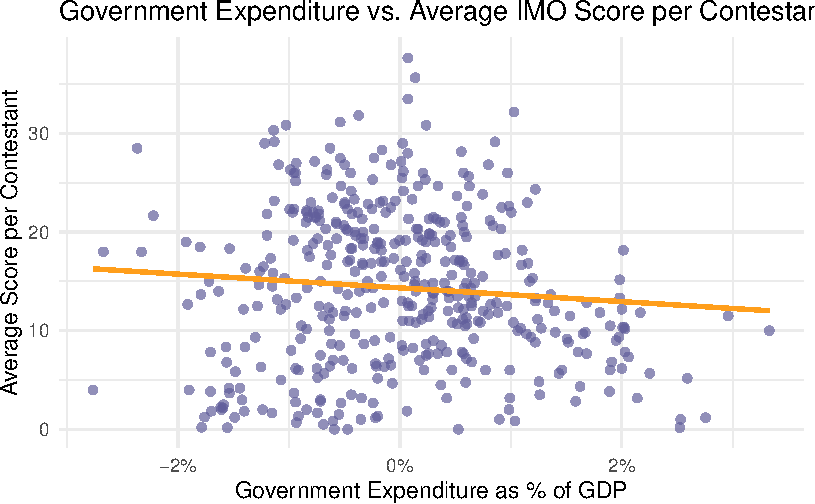
\includegraphics{proj_EDA_f24_sbekova_files/figure-pdf/unnamed-chunk-4-1.pdf}

Interpretation: The plot indicates that government expenditure on
education as a percentage of GDP does not have a significant correlation
with average IMO scores. This suggests that simply increasing spending
may not lead to better performance in mathematics competitions.

\subsection{2.Line Plot: Medal Counts of the Top 3 Countries in 2019
Over the Period
2009--2019}\label{line-plot-medal-counts-of-the-top-3-countries-in-2019-over-the-period-20092019}

This line plot displays the total number of medals won by the top 3
countries from 2009 to 2019, selected based on their medal counts in
2019. Each line represents a country and tracks its medal achievements
over time. The colors of the lines correspond to different countries,
and the labels for each country are positioned next to the last point
(2019) for easy identification. This visualization allows us to observe
the trend and consistency of each country's performance in terms of
medal counts over the 10-year period.

\begin{Shaded}
\begin{Highlighting}[]
\FunctionTok{library}\NormalTok{(ggrepel)}
\CommentTok{\#| message: false}
\CommentTok{\#| warning: false}

\CommentTok{\# 1) Selecting the top 3 countries by the number of medals in 2019}
\NormalTok{top\_countries\_2019 }\OtherTok{\textless{}{-}}\NormalTok{ train\_data }\SpecialCharTok{|\textgreater{}}
  \FunctionTok{filter}\NormalTok{(year }\SpecialCharTok{==} \DecValTok{2019}\NormalTok{) }\SpecialCharTok{|\textgreater{}}
  \FunctionTok{group\_by}\NormalTok{(country) }\SpecialCharTok{|\textgreater{}}
  \FunctionTok{summarize}\NormalTok{(}\AttributeTok{total\_medals\_2019 =} \FunctionTok{sum}\NormalTok{(awards\_gold }\SpecialCharTok{+}\NormalTok{ awards\_silver }\SpecialCharTok{+}\NormalTok{ awards\_bronze, }\AttributeTok{na.rm =} \ConstantTok{TRUE}\NormalTok{)) }\SpecialCharTok{|\textgreater{}}
  \FunctionTok{arrange}\NormalTok{(}\FunctionTok{desc}\NormalTok{(total\_medals\_2019)) }\SpecialCharTok{|\textgreater{}}
  \FunctionTok{slice\_head}\NormalTok{(}\AttributeTok{n =} \DecValTok{3}\NormalTok{) }\SpecialCharTok{|\textgreater{}}
  \FunctionTok{pull}\NormalTok{(country)}

\CommentTok{\# 2) Filtering data for the selected countries from 2009 to 2019}
\NormalTok{medal\_data }\OtherTok{\textless{}{-}}\NormalTok{ train\_data }\SpecialCharTok{|\textgreater{}}
  \FunctionTok{filter}\NormalTok{(country }\SpecialCharTok{\%in\%}\NormalTok{ top\_countries\_2019, year }\SpecialCharTok{\textgreater{}=} \DecValTok{2009}\NormalTok{, year }\SpecialCharTok{\textless{}=} \DecValTok{2019}\NormalTok{) }\SpecialCharTok{|\textgreater{}}
  \FunctionTok{group\_by}\NormalTok{(year, country) }\SpecialCharTok{|\textgreater{}}
  \FunctionTok{summarize}\NormalTok{(}\AttributeTok{total\_medals =} \FunctionTok{sum}\NormalTok{(awards\_gold }\SpecialCharTok{+}\NormalTok{ awards\_silver }\SpecialCharTok{+}\NormalTok{ awards\_bronze, }\AttributeTok{na.rm =} \ConstantTok{TRUE}\NormalTok{)) }\SpecialCharTok{|\textgreater{}}
  \FunctionTok{ungroup}\NormalTok{()}
\end{Highlighting}
\end{Shaded}

\begin{verbatim}
`summarise()` has grouped output by 'year'. You can override using the
`.groups` argument.
\end{verbatim}

\begin{Shaded}
\begin{Highlighting}[]
\CommentTok{\# Set colors for each country}
\NormalTok{country\_colors }\OtherTok{\textless{}{-}} \FunctionTok{setNames}\NormalTok{(}\FunctionTok{c}\NormalTok{(}\StringTok{"\#615e9b"}\NormalTok{, }\StringTok{"\#ff9e1b"}\NormalTok{, }\StringTok{"\#44693d"}\NormalTok{), top\_countries\_2019)}

\CommentTok{\# Plot the graph}
\FunctionTok{ggplot}\NormalTok{(medal\_data, }\FunctionTok{aes}\NormalTok{(}\AttributeTok{x =}\NormalTok{ year, }\AttributeTok{y =}\NormalTok{ total\_medals, }\AttributeTok{color =}\NormalTok{ country, }\AttributeTok{group =}\NormalTok{ country)) }\SpecialCharTok{+}
  \FunctionTok{geom\_line}\NormalTok{(}\AttributeTok{size =} \FloatTok{1.5}\NormalTok{) }\SpecialCharTok{+} \CommentTok{\# Line for each country}
  \FunctionTok{geom\_point}\NormalTok{(}\AttributeTok{size =} \DecValTok{3}\NormalTok{) }\SpecialCharTok{+} \CommentTok{\# Points on the lines}
  \FunctionTok{scale\_color\_manual}\NormalTok{(}\AttributeTok{values =}\NormalTok{ country\_colors) }\SpecialCharTok{+}
  \FunctionTok{scale\_x\_continuous}\NormalTok{(}\AttributeTok{breaks =} \FunctionTok{seq}\NormalTok{(}\DecValTok{2009}\NormalTok{, }\DecValTok{2019}\NormalTok{, }\AttributeTok{by =} \DecValTok{1}\NormalTok{), }\AttributeTok{labels =} \FunctionTok{as.character}\NormalTok{(}\FunctionTok{seq}\NormalTok{(}\DecValTok{2009}\NormalTok{, }\DecValTok{2019}\NormalTok{, }\AttributeTok{by =} \DecValTok{1}\NormalTok{))) }\SpecialCharTok{+}
  \FunctionTok{labs}\NormalTok{(}
    \AttributeTok{title =} \StringTok{"Medal Counts of the Top 3 Countries in 2019 "}\NormalTok{,}
    \AttributeTok{subtitle =} \StringTok{"Over the Period 2009–2019"}\NormalTok{,}
    \AttributeTok{x =} \StringTok{"Year"}\NormalTok{,}
    \AttributeTok{y =} \StringTok{"Total Medals"}\NormalTok{,}
    \AttributeTok{color =} \StringTok{"Country"}
\NormalTok{  ) }\SpecialCharTok{+}
  \FunctionTok{theme\_minimal}\NormalTok{() }\SpecialCharTok{+}
  \FunctionTok{theme}\NormalTok{(}
    \AttributeTok{plot.title =} \FunctionTok{element\_text}\NormalTok{(}\AttributeTok{size =} \DecValTok{16}\NormalTok{, }\AttributeTok{face =} \StringTok{"bold"}\NormalTok{, }\AttributeTok{hjust =} \FloatTok{0.5}\NormalTok{),}
    \AttributeTok{axis.title =} \FunctionTok{element\_text}\NormalTok{(}\AttributeTok{size =} \DecValTok{12}\NormalTok{),}
    \AttributeTok{axis.text =} \FunctionTok{element\_text}\NormalTok{(}\AttributeTok{size =} \DecValTok{10}\NormalTok{),}
    \AttributeTok{panel.grid.major =} \FunctionTok{element\_line}\NormalTok{(}\AttributeTok{color =} \StringTok{"gray80"}\NormalTok{, }\AttributeTok{size =} \FloatTok{0.5}\NormalTok{),}
    \AttributeTok{panel.grid.minor =} \FunctionTok{element\_blank}\NormalTok{(),}
    \AttributeTok{legend.position =} \StringTok{"none"} \CommentTok{\# Remove legend for cleaner design}
\NormalTok{  ) }\SpecialCharTok{+}
 \CommentTok{\# Add annotations for each country next to the latest values}
  \FunctionTok{geom\_text\_repel}\NormalTok{(}\AttributeTok{data =}\NormalTok{ medal\_data }\SpecialCharTok{\%\textgreater{}\%} \FunctionTok{filter}\NormalTok{(year }\SpecialCharTok{==} \DecValTok{2019}\NormalTok{), }
                  \FunctionTok{aes}\NormalTok{(}\AttributeTok{label =}\NormalTok{ country), }
                  \AttributeTok{nudge\_x =} \FloatTok{0.9}\NormalTok{, }\CommentTok{\# Slightly shift text to the right}
                  \AttributeTok{direction =} \StringTok{"y"}\NormalTok{, }\CommentTok{\# Repel text in the y direction}
                  \AttributeTok{size =} \DecValTok{3}\NormalTok{, }\AttributeTok{fontface =} \StringTok{"bold"}\NormalTok{, }\AttributeTok{color =}\NormalTok{ country\_colors)}
\end{Highlighting}
\end{Shaded}

\begin{verbatim}
Warning: Using `size` aesthetic for lines was deprecated in ggplot2 3.4.0.
i Please use `linewidth` instead.
\end{verbatim}

\begin{verbatim}
Warning: The `size` argument of `element_line()` is deprecated as of ggplot2 3.4.0.
i Please use the `linewidth` argument instead.
\end{verbatim}

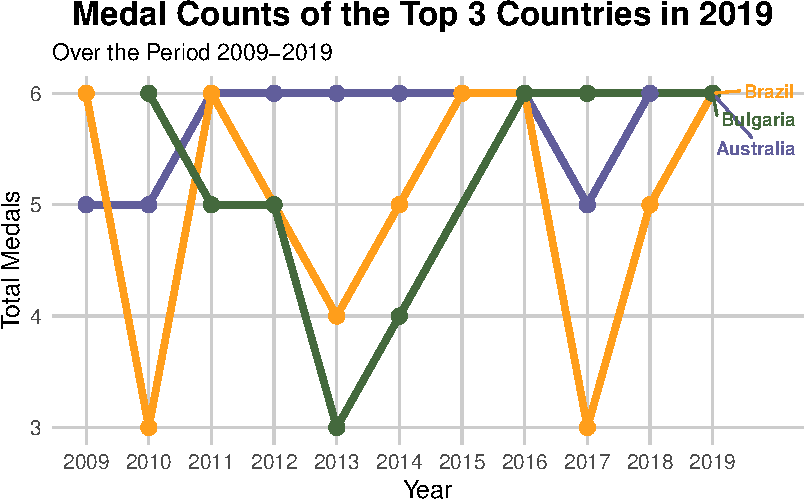
\includegraphics{proj_EDA_f24_sbekova_files/figure-pdf/unnamed-chunk-5-1.pdf}

\subsection{3.Density plot: Distribution of Average IMO Scores by
Literacy Rate
Ranges}\label{density-plot-distribution-of-average-imo-scores-by-literacy-rate-ranges}

\begin{Shaded}
\begin{Highlighting}[]
\CommentTok{\# Density plot showing the distribution of average scores by literacy rate}
\FunctionTok{ggplot}\NormalTok{(train\_data, }\FunctionTok{aes}\NormalTok{(}\AttributeTok{x =}\NormalTok{ average\_score\_per\_contestant, }\AttributeTok{fill =} \FunctionTok{cut}\NormalTok{(Value\_literacy\_rate, }\AttributeTok{breaks =} \FunctionTok{seq}\NormalTok{(}\DecValTok{90}\NormalTok{, }\DecValTok{100}\NormalTok{, }\AttributeTok{by =} \DecValTok{2}\NormalTok{)))) }\SpecialCharTok{+}
  \FunctionTok{geom\_density}\NormalTok{(}\AttributeTok{alpha =} \FloatTok{0.6}\NormalTok{) }\SpecialCharTok{+}
  \FunctionTok{scale\_fill\_brewer}\NormalTok{(}\AttributeTok{palette =} \StringTok{"Blues"}\NormalTok{, }\AttributeTok{name =} \StringTok{"Literacy Rate Range (\%)"}\NormalTok{) }\SpecialCharTok{+}
  \FunctionTok{labs}\NormalTok{(}
    \AttributeTok{title =} \StringTok{"Distribution of Average IMO Scores by Literacy Rate Ranges"}\NormalTok{,}
    \AttributeTok{x =} \StringTok{"Average Score per Contestant"}\NormalTok{,}
    \AttributeTok{y =} \StringTok{"Density"}
\NormalTok{  ) }\SpecialCharTok{+}
  \FunctionTok{theme\_minimal}\NormalTok{()}
\end{Highlighting}
\end{Shaded}

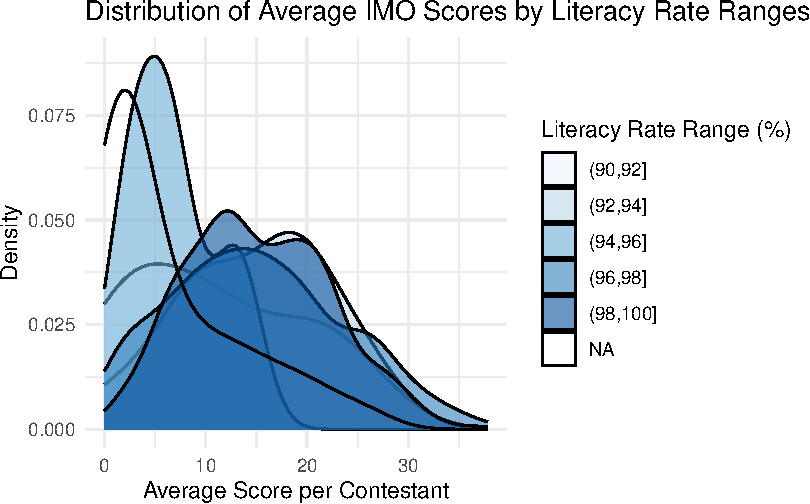
\includegraphics{proj_EDA_f24_sbekova_files/figure-pdf/unnamed-chunk-6-1.pdf}

Interpretation:

The plot suggests that literacy rate does not strongly impact the
distribution of average IMO scores per contestant. Countries with both
lower and higher literacy rates show similar distributions of average
scores, implying that literacy rate alone does not significantly
influence IMO performance.

\subsection{4.Boxplot: Compares the average IMO scores between countries
with and without female team
members:}\label{boxplot-compares-the-average-imo-scores-between-countries-with-and-without-female-team-members}

\begin{Shaded}
\begin{Highlighting}[]
\NormalTok{train\_data\_fem }\OtherTok{\textless{}{-}}\NormalTok{ train\_data }\SpecialCharTok{|\textgreater{}}
  \FunctionTok{mutate}\NormalTok{(}
    \AttributeTok{team\_size\_female =} \FunctionTok{ifelse}\NormalTok{(}\FunctionTok{is.na}\NormalTok{(team\_size\_female), }\DecValTok{0}\NormalTok{, team\_size\_female), }\CommentTok{\# Treat NA as 0}
    \AttributeTok{has\_female\_team =} \FunctionTok{ifelse}\NormalTok{(team\_size\_female }\SpecialCharTok{\textgreater{}} \DecValTok{0}\NormalTok{, }\StringTok{"With Female Team"}\NormalTok{, }\StringTok{"Without Female Team"}\NormalTok{)}
\NormalTok{  )}

\FunctionTok{ggplot}\NormalTok{(train\_data\_fem, }\FunctionTok{aes}\NormalTok{(}\AttributeTok{x =}\NormalTok{ has\_female\_team, }\AttributeTok{y =}\NormalTok{ average\_score\_per\_contestant, }\AttributeTok{fill =}\NormalTok{ has\_female\_team)) }\SpecialCharTok{+}
  \FunctionTok{geom\_boxplot}\NormalTok{() }\SpecialCharTok{+}
  \FunctionTok{labs}\NormalTok{(}
    \AttributeTok{title =} \StringTok{"Average IMO Score per Contestant by Female Team Presence"}\NormalTok{,}
    \AttributeTok{x =} \StringTok{"Female Team Presence"}\NormalTok{,}
    \AttributeTok{y =} \StringTok{"Average Score per Contestant"}
\NormalTok{  ) }\SpecialCharTok{+}
  \FunctionTok{scale\_fill\_manual}\NormalTok{(}\AttributeTok{values =} \FunctionTok{c}\NormalTok{(}\StringTok{"With Female Team"} \OtherTok{=} \StringTok{"\#F28E2B"}\NormalTok{, }\StringTok{"Without Female Team"} \OtherTok{=} \StringTok{"\#4E79A7"}\NormalTok{)) }\SpecialCharTok{+}
  \FunctionTok{theme\_minimal}\NormalTok{() }\SpecialCharTok{+}
  \FunctionTok{theme}\NormalTok{(}\AttributeTok{legend.position =} \StringTok{"none"}\NormalTok{)}
\end{Highlighting}
\end{Shaded}

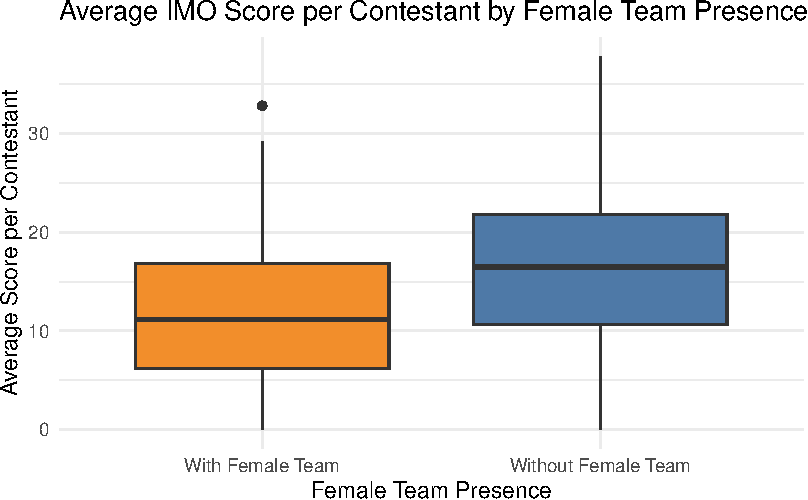
\includegraphics{proj_EDA_f24_sbekova_files/figure-pdf/unnamed-chunk-7-1.pdf}

The plot suggests a slight association between the absence of female
team members and higher average IMO scores, although the difference is
not very large.



\end{document}
